\subsubsection{Actividad2}

\begin{frame}
	\frametitle{\underline{\textbf{Modificación de las variables de una señal periódica}}}
		
	Aprender a variar los componentes básicos de una señal periódica (Amplitud, frecuencia, fase y nivel DC) en GNU Radio.\vspace{2mm}
		
	Es importante saber que:
	
	\begin{enumerate}[1.]
	\item{La forma más simple de representar una señal periódica es una senoidal como se presenta matemáticamente a continuación}\\
	
	$$x(t)=A\sin(2 \pi f + \phi) + K$$\\
	
	En donde:\\
	
	\item{Amplitud ($A$): Es el valor máximo que toma la señal, es decir, la distancia entre el punto máximo de la señal y cero, este punto puede ser tanto positivo como negativo}\\
			
	\item{Frecuencia ($f$): Es el número de ciclos que realiza la señal por unidad de tiempo, esta medida está dada en Hertz (Hz), que equivale a un ciclo por segundo, lo que significa que 80Hz son 80 ciclos por cada segundo que transcurre.}\\

	\end{enumerate}
	\end{frame}
	
	
	\begin{frame}
	\begin{enumerate}[1.]

	\item{La fase ($\phi$): Indica la magnitud de una de variación ciclica, siendo la fracción del período que transcurre desde el instante tomado al estado tomado como referencia, es decir el desplazamiento que tiene una señal en grados con respecto a su referencia, por ejemplo, la señal seno está desfada 90 grados con respecto a la señal coseno.}\\
	
	\item{Nivel DC ($K$): Es el valor medio de la señal, lo que quiere decir que es un voltaje en DC que se le suma a la señal AC, para obtener un desplazamiento en la amplitud de la señal, puede ser tanto positivo como negativo.}\\

	\end{enumerate}
	\end{frame}
	
	
		
	\begin{frame}

	\frametitle{\underline{\textbf{Pistas para la actividad}}}

	Las pistas son:
	\begin{enumerate}[1.]

	\item {Repasar los bloques utilizados en la primer guía "Primeros pasos"}\\
	\item {Debe existir un WX GUI Slider para cada variable que se desee modificar en el osciloscopio.}\\
	\item {Para una mejor apreciación  de los cambios en las variables de la señal se sugiere añadir otra señal que sirva como referencia}\\
	\item {Coherencia entre los tipos de dato entre bloques}\\
	\item {Para variar el nivel DC de la señal, el oscilocopio debe tener la opción "Acopling" en DC}\\
	
	\end{enumerate}
	\end{frame}
	


%\begin{frame}{Primeros pasos }
%\begin{figure}[H]
%	\vspace{-3mm}
%	\centering
%	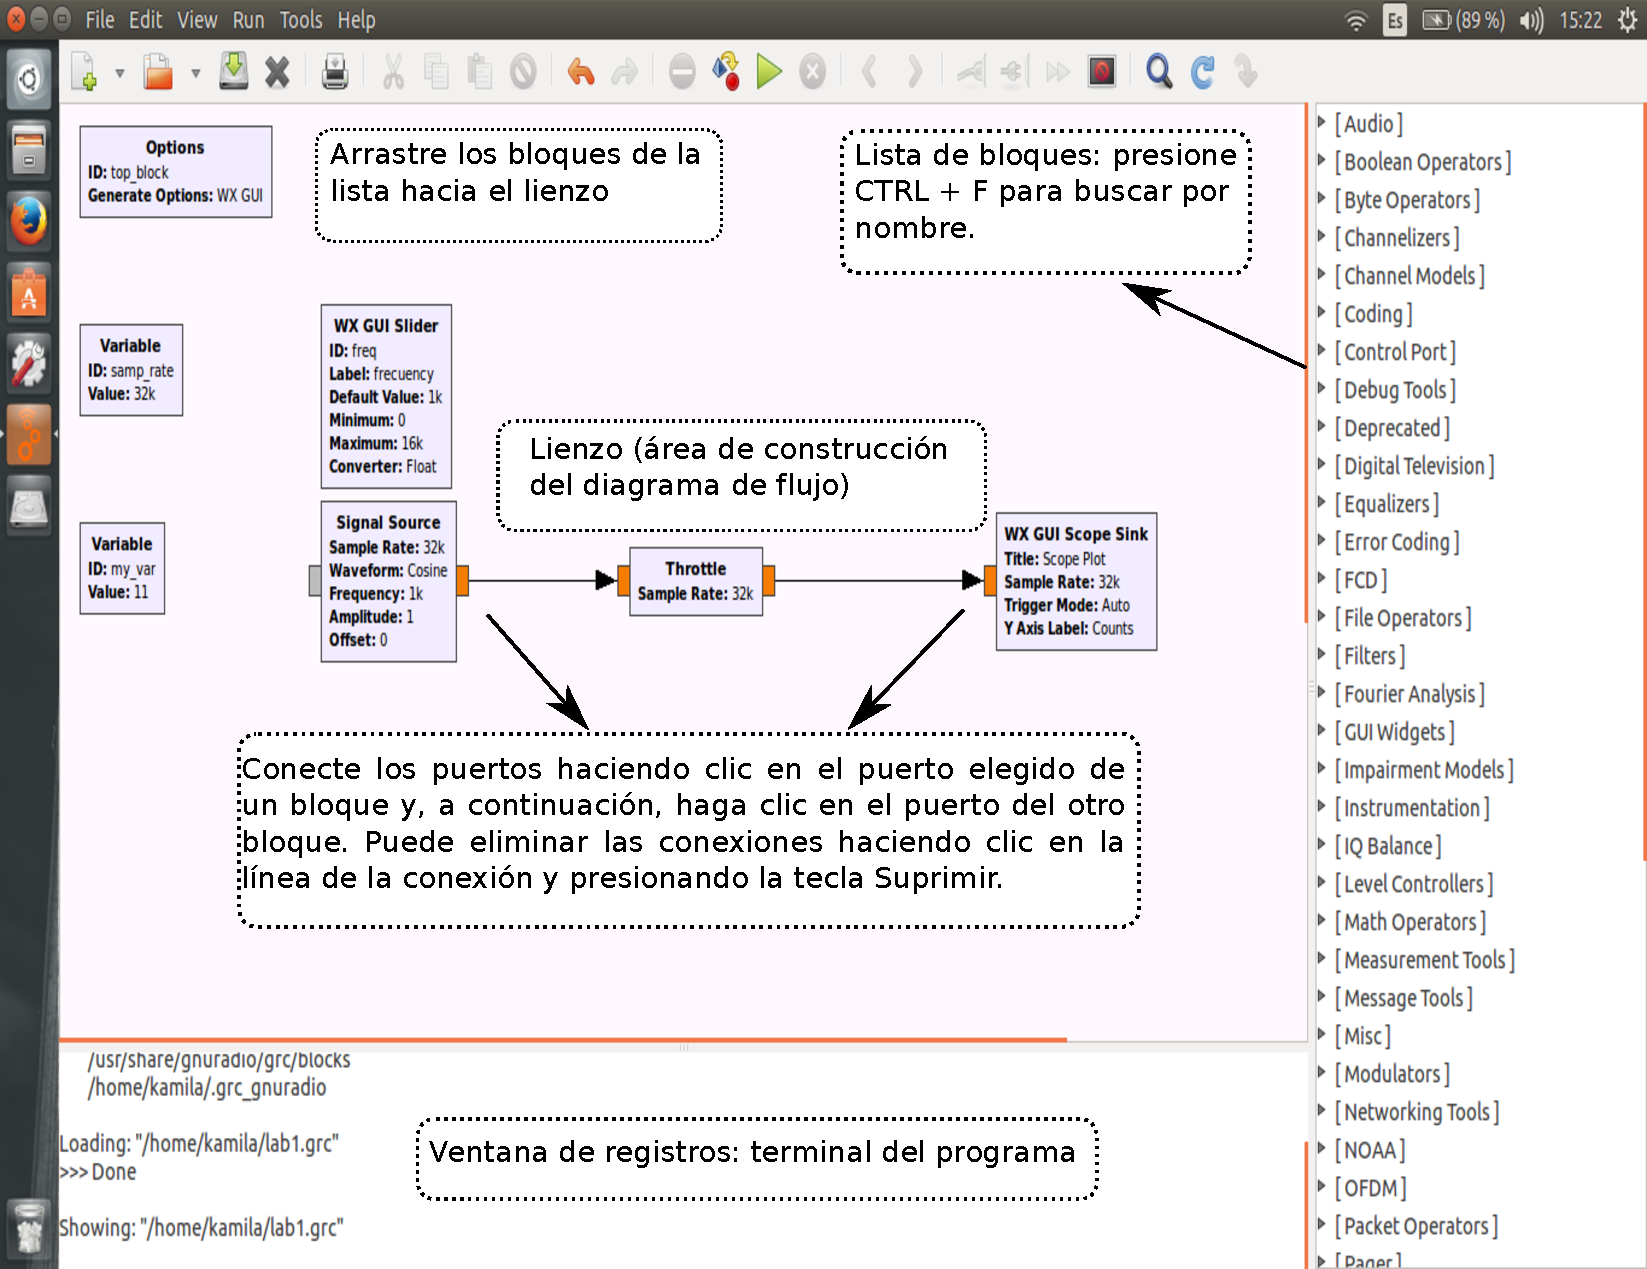
\includegraphics[width=0.9\textwidth]{Actividades2/pdf/lab1_1.pdf}
%\end{figure}
%\end{frame}